\documentclass[a4paper]{article}
\usepackage[a4paper,margin=0mm]{geometry}
\usepackage{fontspec}
\usepackage{unicode-math}
\usepackage{tikz}
\usetikzlibrary{fit,calc,positioning,arrows.meta}
\usepackage[table]{xcolor}
\usepackage[absolute]{textpos}
\usepackage{array}

\setmainfont{Libertinus Serif}
\setsansfont{Libertinus Sans}
\setmathfont{Libertinus Math}

\definecolor{accent}{HTML}{602785}
\definecolor{badge}{HTML}{B8A0C8}
\definecolor{ink}{HTML}{2A2E30}

\setlength{\TPHorizModule}{1mm}
\setlength{\TPVertModule}{1mm}
\setlength{\parindent}{0pt}
\pagestyle{empty}

\newcommand{\topicheader}[2]{%
\begin{textblock*}{194mm}(16mm,10mm)
\begin{tikzpicture}
\node[fill=accent,text=white,font=\sffamily\bfseries\fontsize{13}{13}\selectfont,
      minimum width=9mm,minimum height=9mm,inner sep=0pt] at (4.5mm,-4.5mm) {#1};
\node[font=\sffamily\bfseries\fontsize{15}{16}\selectfont,text=ink,anchor=west] at (12mm,-4.5mm) {#2};
\end{tikzpicture}
\end{textblock*}
\begin{textblock*}{194mm}(16mm,22.5mm)

\begin{tikzpicture}
\fill[accent] (0,0) rectangle (194mm,0.5mm);
\end{tikzpicture}
\end{textblock*}
}

\newcommand{\pagekicker}[1]{%
\begin{textblock*}{100mm}(16mm,25.5mm)
\begin{tikzpicture}
\node[fill=ink,text=white,font=\sffamily\bfseries\fontsize{8}{8}\selectfont,
      inner sep=2.2pt,rounded corners=1pt] {\MakeUppercase{#1}};
\end{tikzpicture}
\end{textblock*}
}

\newcommand{\videobanner}[1]{%
\begin{textblock*}{178mm}(16mm,25.5mm)
\begin{tikzpicture}
\fill[accent] (0,0) rectangle (178mm,-10mm);
\draw[white,line width=0.6pt] (3mm,-1.7mm) rectangle (11.5mm,-8.3mm);
\node[white,font=\sffamily\fontsize{4}{4.4}\selectfont,align=center] at (7.25mm,-5mm) {QR\\CODE};
\node[white,font=\sffamily\bfseries\fontsize{9.5}{11}\selectfont,anchor=west] at (16mm,-5.6mm) {WATCH THE VIDEO BEFORE YOU SOLVE};
\node[white,font=\sffamily\fontsize{7.5}{8}\selectfont,anchor=east] at (174mm,-5.6mm) {YouTube ~\textbullet~ #1};
\end{tikzpicture}
\end{textblock*}
}

\newcommand{\pagefooter}[1]{%
\begin{textblock*}{194mm}(8mm,286.41mm)
  
\begin{tikzpicture}
    \fill[accent] (0,0) rectangle (194mm,0.6mm);
  \end{tikzpicture}
\end{textblock*}
\begin{textblock*}{63.59mm}(8mm,288.27mm)
  {\sffamily\bfseries\color{accent}\fontsize{13}{16}\selectfont SAT 1200+}
\end{textblock*}
\begin{textblock*}{10mm}(188mm,288.27mm)
  \centering{\sffamily\color{accent}\fontsize{14}{16}\selectfont #1}
\end{textblock*}
}

\newcommand{\cardbg}[4]{%
\begin{textblock*}{#3mm}(#1mm,#2mm)
\begin{tikzpicture}
\fill[badge!22,rounded corners=3mm] (0,0) rectangle (#3mm,-#4mm);
\end{tikzpicture}
\end{textblock*}%
}

\newcommand{\pill}[3]{%
\begin{textblock*}{160mm}(#1mm,#2mm)
\begin{tikzpicture}
\node[fill=accent,text=white,anchor=north west,font=\sffamily\bfseries\fontsize{10}{10}\selectfont,
      rounded corners=8pt,inner xsep=5mm,inner ysep=1.8mm] at (0,0) {RULE ~\textperiodcentered~ #3};
\end{tikzpicture}
\end{textblock*}%
}

\arrayrulecolor{accent}
\setlength{\arrayrulewidth}{0.7pt}
\renewcommand{\arraystretch}{1.5}

\begin{document}

% ======================================================================
% PAGE 1
% ======================================================================
\topicheader{1}{Linear Equations \& Inequalities}
\videobanner{Lesson 1}
\pagefooter{7}
\mbox{}%

% ---- CARD 1: Multi-step equations ----
\cardbg{16}{40}{178}{42}
\pill{26}{43}{Multi-step equations (ko'p qadamli tenglama)}

\begin{textblock*}{158mm}(26mm,56mm)
{\fontsize{11}{14}\selectfont\color{ink}
Order: clear fractions $\to$ expand $\to$ collect the variable $\to$ combine
like terms.}
\end{textblock*}

\begin{textblock*}{158mm}(26mm,67mm)
{\fontsize{13}{16}\selectfont
$\dfrac{2}{3}(x+3)=x-1\ \Longrightarrow\ x=9$}
\end{textblock*}

% ---- CARD 2: Sign-flip rule ----
\cardbg{16}{88}{178}{70}
\pill{26}{91}{Sign-flip rule (ishora almashish qoidasi)}

\begin{textblock*}{158mm}(26mm,104mm)
{\fontsize{11}{14}\selectfont
\begin{tabular}{|p{80mm}|>{\centering\arraybackslash}p{70mm}|}
\hline
\rowcolor{accent}
{\color{white}\textbf{Operation}} & {\color{white}\textbf{Sign flips?}} \\ \hline
Add or subtract & No \\ \hline
Multiply / divide by a positive & No \\ \hline
\textbf{Multiply / divide by a negative} & \textbf{Yes} \\ \hline
\end{tabular}}
\end{textblock*}

\begin{textblock*}{158mm}(26mm,146mm)
{\fontsize{13}{16}\selectfont
$-3x+5\le20\ \Longrightarrow\ x\ge-5$}
\end{textblock*}

% ---- CARD 3: Graphing the solution ----
\cardbg{16}{166}{178}{110}
\pill{26}{169}{Graphing the solution}

\begin{textblock*}{158mm}(26mm,182mm)
{\fontsize{11}{14}\selectfont
\begin{tabular}{|>{\centering\arraybackslash}p{20mm}|p{60mm}|p{58mm}|}
\hline
\rowcolor{accent}
{\color{white}\textbf{Sign}} & {\color{white}\textbf{Circle}} & {\color{white}\textbf{Meaning}} \\ \hline
$<$ or $>$ & Open circle & Boundary excluded \\ \hline
$\le$ or $\ge$ & Closed circle & Boundary included \\ \hline
\end{tabular}}
\end{textblock*}

\begin{textblock*}{158mm}(26mm,211mm)
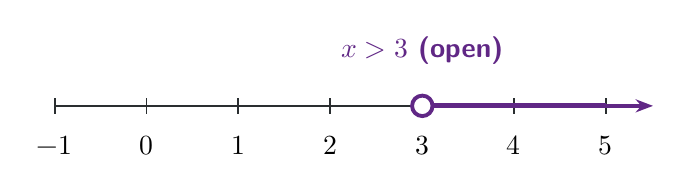
\begin{tikzpicture}[every node/.style={font=\fontsize{10}{10}\selectfont}]
\draw[ink,line width=0.9pt] (0,0) -- (70mm,0);
\foreach \x/\lbl in {0/{-1},11.67/{0},23.3/{1},35/{2},46.7/{3},58.3/{4},70/{5}}{
  \draw[ink,line width=0.7pt] (\x mm,-1mm) -- (\x mm,1mm);
  \node at (\x mm,-5mm) {$\lbl$};
}
\draw[accent,line width=1.8pt] (46.7mm,0) -- (70mm,0);
\draw[accent,line width=1.4pt,-{Stealth[length=2.2mm]}] (68mm,0) -- (76mm,0);
\draw[accent,line width=1.4pt,fill=white] (46.7mm,0) circle (1.3mm);
\node[font=\sffamily\bfseries\fontsize{10}{10}\selectfont,text=accent] at (46.7mm,7mm) {$x>3$ (open)};
\end{tikzpicture}
\end{textblock*}

\begin{textblock*}{158mm}(26mm,236mm)
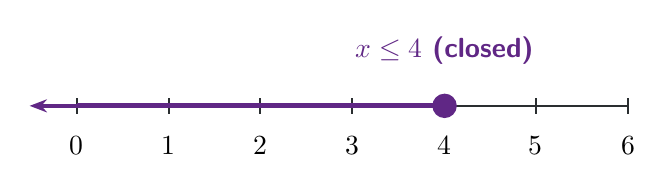
\begin{tikzpicture}[every node/.style={font=\fontsize{10}{10}\selectfont}]
\draw[ink,line width=0.9pt] (0,0) -- (70mm,0);
\foreach \x/\lbl in {0/{0},11.67/{1},23.3/{2},35/{3},46.7/{4},58.3/{5},70/{6}}{
  \draw[ink,line width=0.7pt] (\x mm,-1mm) -- (\x mm,1mm);
  \node at (\x mm,-5mm) {$\lbl$};
}
\draw[accent,line width=1.8pt] (0,0) -- (46.7mm,0);
\draw[accent,line width=1.4pt,-{Stealth[length=2.2mm]}] (2mm,0) -- (-6mm,0);
\draw[accent,line width=1.4pt,fill=accent] (46.7mm,0) circle (1.3mm);
\node[font=\sffamily\bfseries\fontsize{10}{10}\selectfont,text=accent] at (46.7mm,7mm) {$x\le4$ (closed)};
\end{tikzpicture}
\end{textblock*}

\clearpage

% ======================================================================
% PAGE 2
% ======================================================================
\topicheader{1}{Linear Equations \& Inequalities}
\pagekicker{Rules sheet -- 2/2}
\pagefooter{8}
\mbox{}%

% ---- CARD 4: Compound inequalities ----
\cardbg{16}{33}{178}{130}
\pill{26}{36}{Compound inequalities (qo'shma tengsizlik)}

\begin{textblock*}{158mm}(26mm,49mm)
{\fontsize{11}{14}\selectfont\textbf{``And''} -- one operation, all three parts.}
\end{textblock*}

\begin{textblock*}{158mm}(26mm,59mm)
{\fontsize{13}{16}\selectfont $-3<x+1\le5\ \Longrightarrow\ -4<x\le4$}
\end{textblock*}

\begin{textblock*}{158mm}(26mm,74mm)
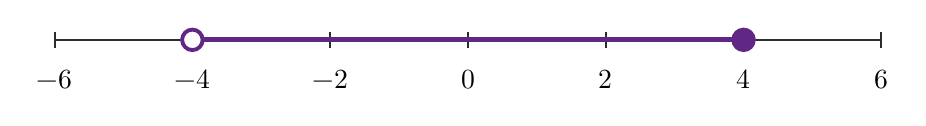
\begin{tikzpicture}[every node/.style={font=\fontsize{10}{10}\selectfont}]
\draw[ink,line width=0.9pt] (0,0) -- (105mm,0);
\foreach \x/\lbl in {0/{-6},17.5/{-4},35/{-2},52.5/{0},70/{2},87.5/{4},105/{6}}{
  \draw[ink,line width=0.7pt] (\x mm,-1mm) -- (\x mm,1mm);
  \node at (\x mm,-5mm) {$\lbl$};
}
\draw[accent,line width=1.8pt] (17.5mm,0) -- (87.5mm,0);
\draw[accent,line width=1.4pt,fill=white] (17.5mm,0) circle (1.3mm);
\draw[accent,line width=1.4pt,fill=accent] (87.5mm,0) circle (1.3mm);
\end{tikzpicture}
\end{textblock*}

\begin{textblock*}{158mm}(26mm,100mm)
{\fontsize{11}{14}\selectfont\textbf{``Or''} -- each part solved separately.}
\end{textblock*}

\begin{textblock*}{158mm}(26mm,110mm)
{\fontsize{13}{16}\selectfont $2x+1<-3$ or $2x+1>7\ \Longrightarrow\ x<-2$ or $x>3$}
\end{textblock*}

\begin{textblock*}{158mm}(26mm,125mm)
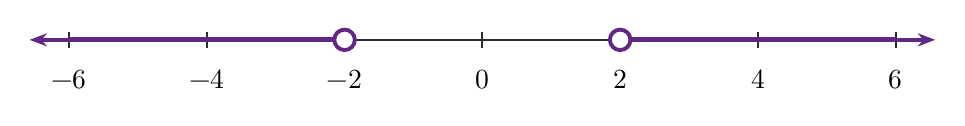
\begin{tikzpicture}[every node/.style={font=\fontsize{10}{10}\selectfont}]
\draw[ink,line width=0.9pt] (0,0) -- (105mm,0);
\foreach \x/\lbl in {0/{-6},17.5/{-4},35/{-2},52.5/{0},70/{2},87.5/{4},105/{6}}{
  \draw[ink,line width=0.7pt] (\x mm,-1mm) -- (\x mm,1mm);
  \node at (\x mm,-5mm) {$\lbl$};
}
\draw[accent,line width=1.8pt] (0,0) -- (35mm,0);
\draw[accent,line width=1.4pt,-{Stealth[length=2.2mm]}] (3mm,0) -- (-5mm,0);
\draw[accent,line width=1.4pt,fill=white] (35mm,0) circle (1.3mm);
\draw[accent,line width=1.8pt] (70mm,0) -- (105mm,0);
\draw[accent,line width=1.4pt,-{Stealth[length=2.2mm]}] (102mm,0) -- (110mm,0);
\draw[accent,line width=1.4pt,fill=white] (70mm,0) circle (1.3mm);
\end{tikzpicture}
\end{textblock*}

\begin{textblock*}{158mm}(26mm,150mm)
{\fontsize{10}{13}\selectfont\color{black!55}\itshape
Operation applies to all three parts of an ``and'' inequality -- not just one.}
\end{textblock*}

% ---- CARD 5: Interval notation ----
\cardbg{16}{173}{178}{42}
\pill{26}{176}{Interval notation (oraliq belgilash)}

\begin{textblock*}{158mm}(26mm,189mm)
{\fontsize{10.5}{13}\selectfont\color{ink}
Traditional textbooks: semicolon. SAT / English sources: comma.}
\end{textblock*}

\begin{textblock*}{158mm}(26mm,200mm)
{\fontsize{13}{16}\selectfont
Traditional: $(2;\ 5]$ \hspace{15mm} SAT: $(2,\ 5]$}
\end{textblock*}

\end{document}
